\chapter{Passive Filters}
In the last chapter, I used an example to demonstrate the mechanics of determining unknown quantities in AC circuits. As part of that analysis, we saw that the source frequency has a great impact on the parameters of the function of interest. In practice, circuits are commonly designed to exploit the frequency-dependence of capacitors and inductors. In this chapter, we will examine several configurations of circuit elements that are designed to manipulate a time-varying voltage in a frequency-dependent way. As I discuss these circuits, I may use some language that is not familiar to you. Let me define a few terms now so you will know to what I am referring. 
\par
First, a \textbf{signal} is a time-dependent voltage or current that carries some information. Think about music you listen to through headphones; the time-varying voltage that carries that music to your headphones is an example of a signal.
\par
Next, the \textbf{frequency content} or \textbf{frequency spectrum} of a signal is all of the different frequencies that are contained in a signal. Again, music is made of a continuum of frequency content, with its spectrum spanning from less than 100Hz to about 20kHz. 
\par
When I refer to \textbf{filtering} a signal, I mean that I will be adjusting the amplitude of a certain range of frequencies contained within that signal. With music, an example of this is when the bass or the treble knobs of an equalizer are adjusted. 
\par
Finally, \textbf{attenuation} means a decrease in amplitude. To attenuate a certain range of frequencies is to diminish the amplitude of those frequencies.

\section{Frequency Response}
So far, we have considered circuits with a single-frequency source. In this chapter, we will leave the exact parameters of the source out of the analysis, and instead we will treat frequency as an independent variable in our calculations. Consider the diagram of Figure \ref{inOutSignalBox}.

\begin{figure}[h!]
\centering
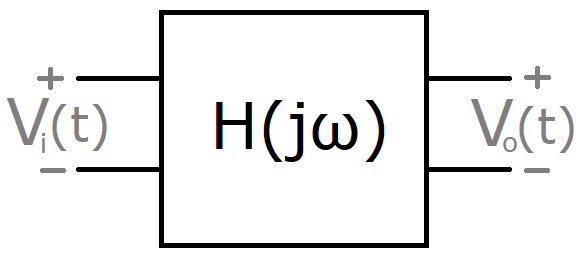
\includegraphics[width=10cm]{figures/signalInOutBox.png}
\caption{A generic frequency-dependent circuit with an input and an output voltage.}
\label{inOutSignalBox}
\end{figure}

This box takes a voltage signal $v_i(t)$ as its input and presents a voltage signal $v_o(t)$ at its output terminals. The output voltage, $V_o(t)$ is related to $V_i(t)$ by H($j\omega$), which is known as the \textbf{frequency response} of the system in the box. Note that frequency response is not a function of time, but frequency. In general, for any system with an input voltage and an output voltage, the definition for frequency response is
$$
\mathnormal{H(j\omega)} = \frac{V_o}{V_i}
$$
Where $V_o$ and $V_i$ represent the phasor forms for these voltages. 
\par
Before we get into specifics, let's look at the circuit of Figure \ref{voltageDivWithBoxElements}. We have very limited information here, but we can still express the frequency response of the circuit in terms of the impedances given. 
\begin{figure}[h!]
\centering
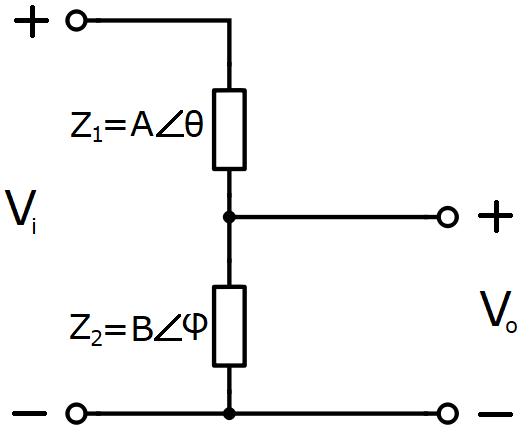
\includegraphics[width=10cm]{figures/voltageDivBoxes.png}
\caption{A generic voltage divider comprised of two sections of elements each with their own impedance.}
\label{voltageDivWithBoxElements}
\end{figure}
Using the voltage divider rule, we know how to relate the voltage across Z$_2$ ($V_o$) to the input voltage $V_i$:
$$
V_o = V_i\cdot\left(\frac{Z_2}{Z_1+Z_2}\right)
$$
We aren't interested in an exact value for $V_o$, but we can use this expression to find the frequency response for the circuit by dividing both sides by $V_i$:
$$
H(j\omega) = \left(\frac{Z_2}{Z_1+Z_2}\right)
$$
If we had specific values for these impedances, we could analyze the resulting frequency response to determine the filtering behavior for the circuit. In the following sections, we will do this analysis with several common passive filters that use just resistors, capacitors, and inductors.

\section{RC High-Pass and Low-Pass Filters}
Consider the circuit of Figure \ref{RC_HP}. This is just a voltage divider with a resistor and a capacitor, and the output of the circuit is the voltage across the resistor. 
\begin{figure}[h!]
\centering
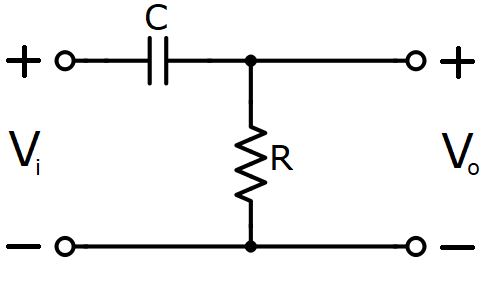
\includegraphics[width=10cm]{figures/RC_HP.png}
\caption{A voltage divider with a resistor and a capacitor.}
\label{RC_HP}
\end{figure}
As we did before, we can determine the frequency response for this system by using the voltage divider rule:
$$
H(j\omega) = \frac{Z_R}{Z_R+Z_C} = \frac{R}{R+(1/j\omega C)}
$$
This is a function of frequency like we want, but its current form is gross. We need to make it look better so we can more easily analyze the behavior of the system. One way to improve it is to get rid of the fraction in the denominator. To do this, we will multiply both the numerator and the denominator by $j\omega C$:\footnote{I call this process ``multiplying by a fancy 1'', because we are really just multiplying the whole frequency response by 1, but it's a form of 1 that works to our advantage.}
$$
H(j\omega) = \frac{R}{R+(1/j\omega C)}\cdot\frac{j\omega C}{j\omega C}
$$
$$
= \frac{j\omega RC}{j\omega RC +1}
$$
\par
This is a much more satisfying form of the frequency response for this circuit. Now that we have determined the frequency response, let's analyze the behavior of this circuit at different driving frequencies. Of course, there is an infinite range of frequencies, but we can get a sense of the behavior of a circuit by determining what happens to the frequency response at $\omega=0$ and as $\omega\rightarrow\infty$:
$$
\textnormal{For }\omega=0\textnormal{: }H(0) = \frac{0}{1} = 0
$$
$$
\textnormal{For }\omega\rightarrow\infty\textnormal{: }H(j\infty) = \frac{j\infty}{j\infty+1} \approx 1
$$
So, for $\omega=0$, the output voltage is 0. This is akin to connecting a DC source to the input for the circuit. This tells us that the filter in question preferrentially attenuates signals of lower frequency. Conversely, as the frequency approaches infinity, the frequency response approaches 1, which means that the output voltage is equal to the input voltage. These two conditions for the frequency response tell us that this circuit is a \textbf{high-pass filter}, because it allows signals of high frequency to pass through unchanged, while lower frequencies are attenuated.
\begin{figure}[h!]
\centering
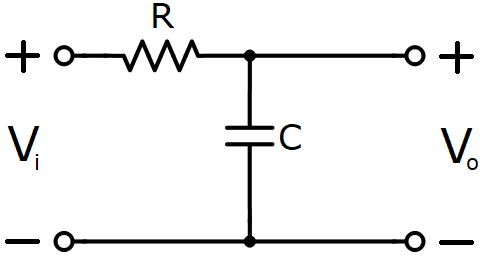
\includegraphics[width=10cm]{figures/RC_LP.png}
\caption{Another voltage divider with a resistor and a capacitor.}
\label{RC_LP}
\end{figure}
\par
Now let's analyze the circuit of Figure \ref{RC_LP}. This is a voltage divider with just a resistor and capacitor, too, but in this system we are taking the output $V_o$ from across the capacitor. This results in the following frequency response:
$$
H(j\omega) = \frac{Z_C}{Z_R+Z_C} = \frac{\frac{1}{j\omega C}}{R+(1/j\omega C)}
$$
Again, we will get rid of the fractions in the numerator and denominator of this expression by multiplying both by $j\omega C$:
$$
H(j\omega) = \frac{\frac{1}{j\omega C}}{R+(1/j\omega C)}\cdot\frac{j\omega C}{j\omega C} 
$$
$$
= \frac{1}{j\omega RC + 1}
$$
\par
Now let's consider the frequency response for the cases we considered before. If $\omega=0$, H(j0)=1. This tells us that when the frequency of the input signal is low, the output is roughly equal to the input. However, when $\omega\rightarrow\infty$, H(j$\infty$)$\approx$ 0. This means that as the frequency of the input signal increases, the amplitude of the output voltage decreases. We call this circuit a \textbf{low-pass filter}, because if the input signal frequency is low, it will be allowed to pass through the filter without its amplitude decreasing.
\par
For both of these types of filters, it would be nice to have a way to quantify their frequency responses without simply citing a frequency-dependent function. Fortunately, we can describe their behavior in terms of a single \textbf{cutoff frequency}, $\omega_c$. This is defined as follows:
$$
|H(j\omega_c)| = \frac{1}{\sqrt{2}}
$$
Why $\sqrt{2}$? Remember the form of Watt's law that says power delivered to an element is proportional to the voltage across that element squared? Well, if the frequency response of one of these filters is equal to $\frac{1}{\sqrt{2}}$, that means the output voltage can deliver just half the amount of power to a load that could have been delivered by the input voltage. Because of this, the cutoff frequency is also called the \textbf{half-power frequency}. Below, I derive the definition of the cutoff frequency using the frequency response of the low-pass filter:
$$
\frac{1}{\sqrt{2}} = |H(j\omega_c)| = \left|\frac{1}{j\omega_c RC +1}\right|
$$
$$
\sqrt{2} = |(j\omega_c RC +1)| = \sqrt{(1 + j\omega_c RC)\cdot(1 - j\omega_c RC)}
$$
$$
= \sqrt{(1 \cancel{+ j\omega_c RC - j\omega_c RC} - \cancelto{-1}{j^2}\omega_c^2(RC)^2)} = \sqrt{1+ \omega_c^2 (RC)^2}
$$
$$
2 = 1+\omega_c^2(RC)^2
$$
$$
\frac{1}{(RC)^2}=\omega_c^2
$$
$$
\omega_c=\frac{1}{RC}
$$
While we derived this definition using the frequency response for the low-pass filter, both high-pass and low-pass filter types have the same definition for cutoff frequency. When describing a filter circuit in practice, we will usually give a cutoff frequency and a filter type rather than citing the full frequency response expression.


%Both the high-pass and the low-pass filters are just voltage dividers comprised of a single resistor in series with a single capacitor. The main difference between these two filters is the element across which the output voltage is measured. 
%\par 
%Let's add the frequency responses for both of these filters together; I'll use subscripts ``HP'' and ``LP'' to distinguish between the frequency response of the high-pass filter and low-pass filter, respectively:
%$$
%H_{HP}(j\omega) + H_{LP}(j\omega) = \frac{j\omega RC}{j\omega RC +1} + \frac{1}{j\omega RC + 1} = \frac{j\omega RC + 1}{j\omega RC + 1} = 1
%$$
%The fact that the sum of the two frequency responses for these systems is 1 tells us that their respective outputs are complimentary; if we drove both circuits with the same input signal, we could reproduce the input signal by summing the output signals from both systems. 

\section{RLC Band-Pass and Band-Stop Filters}
High- and low-pass filters are the most commonly seen passive filter circuits in practice. Sometimes a circuit is needed that will either allow just a single frequency to pass through, or cut a single frequency out of the input. To accomplish these tasks, a \textbf{Band-Pass} or a \textbf{Band-Stop} Filter, respectively, could be used.
\begin{figure}[h!]
\centering
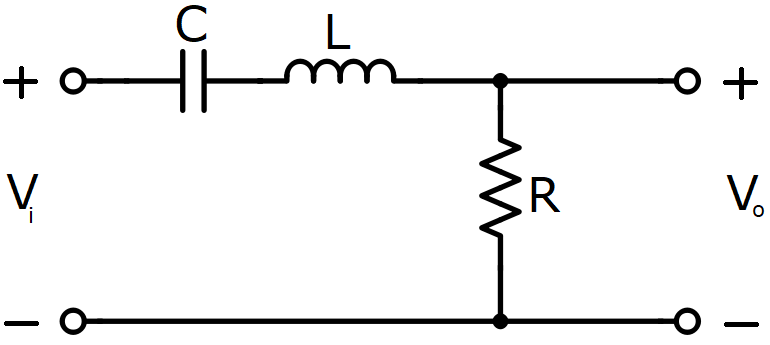
\includegraphics[width=10cm]{figures/BPfilter.png}
\caption{A voltage divider comprised of a capacitor, inductor, and resistor.}
\label{RLC_BP}
\end{figure}
\par
Consider the circuit in Figure \ref{RLC_BP}. This circuit is a voltage divider comprised of a capacitor, an inductor, and a resistor. We can again define $H(j\omega)$ using the voltage divider rule as follows:
$$
H(j\omega) = \frac{Z_R}{Z_R+Z_L+Z_C} = \frac{R}{R + j\omega L+\frac{1}{j\omega C}} = \frac{R}{R + j\left(\omega L-\frac{1}{\omega C}\right)}
$$
This frequency response differs from those of the high- and low- pass filters in one major way---its imaginary component is the difference of two frequency-dependent terms. This means that there is a particular input frequency (which we will call the \textbf{resonant frequency} for the circuit, $\omega_0$) that will cause those two terms to cancel each other. If that were the case, the amplitude of the frequency response would be 
$$
\left|H(j\omega_0)\right|=\left|\frac{R}{R + j\cancelto{0}{\left(\omega_0\cdot L-\frac{1}{\omega_0\cdot C}\right)}}\right| = 1
$$
This demonstrates that at that particular frequency, the input would pass through to the output without losing any amplitude. 
\par
Now let's determine what would happen at the two extreme ends of the valid frequency range. If the frequency were 0, the amplitude of the frequency response would be
$$
\left|H(j\cdot0)\right|=\left|\frac{R}{R + j\left(0\cdot L-\cancelto{\infty}{\frac{1}{0\cdot C}}\right)}\right| = 0 
$$
If instead, the frequency approaches infinity, the frequency response would be
$$
\left|H(j\cdot\infty)\right|=\left|\frac{R}{R + j\left(\infty\cdot L-\cancelto{0}{\frac{1}{\infty\cdot C}}\right)}\right| = 0 
$$
In both of these cases, the output amplitude is diminished to 0. We can extrapolate these three cases to conclude that this filter only allows some frequencies close to the resonant frequency, $\omega_0$, to pass through to the output, and the rest of the frequency range is attenuated (i.e., cut out). This circuit is called a \textbf{Band-Pass Filter}, because it only allows a ``band'' of frequencies to pass through from input to output. 
\par
A band-pass filter can, of course, be characterized with its frequency response formula, but in practice we use its resonant frequency and its \textbf{bandwidth} to describe its behavior. To determine its resonant frequency, we set the imaginary component to zero and then solve that equation for $\omega_0$:
$$
\omega_0 L-\frac{1}{\omega_0 C} = 0
$$
$$
\omega_0 L = \frac{1}{\omega_0 C}
$$
$$
\omega_0^2 = \frac{1}{LC}
$$
$$
\omega_0 = \frac{1}{\sqrt{LC}}
$$
The next quantity we want to determine is the \textbf{bandwidth} of the circuit. The bandwidth is a measure of how dramatically the output of the filter attenuates as the input frequency is swept off of the resonant frequency. We call this the ``bandwidth'' because it is the actual width (in dimensions of frequency) of the band of frequencies that are passed through the circuit. Quantitatively, the bandwidth of a band-pass filter is simply the difference between its two half-power frequencies. We found the half-power frequency for the high-pass and low-pass filters in the last section, but each of those filters only had single half-power frequency. The band-pass filter has two such frequencies. I will not derive them here, because it requires a tedious calculation, and nobody wants that\footnote{If you do want to see this derivation, you can find it online, or better yet, do it yourself! But be prepared with the quadratic formula and lots of paper.}. The \textbf{bandwidth} for the filter is
$$
\beta = \frac{R}{L}
$$
\par
This expression for the bandwidth tells us that if the resistor in the filter is of a high value, the pass-band of frequencies is wide, whereas if the resistance is small, the pass-band is narrow. Note that the bandwidth is not dependent on the value of the capacitor.
\par
The last type of filter I will introduce in this chapter is the \textbf{Band-Stop Filter}. Its general form is shown in Figure \ref{RLC_BS}. 
\begin{figure}[h!]
\centering
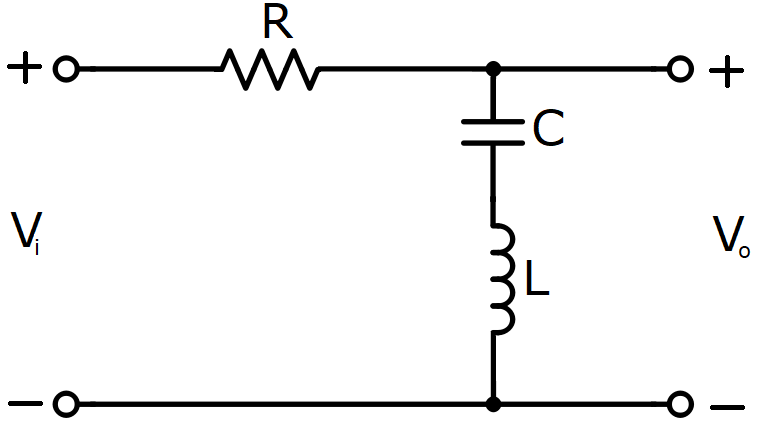
\includegraphics[width=10cm]{figures/BSfilter.png}
\caption{Another voltage divider comprised of a capacitor, inductor, and resistor.}
\label{RLC_BS}
\end{figure}
Does this circuit look familiar? Hopefully by now you have noticed that all our filters are really just voltage dividers. I told you those were useful!
\par
The band-stop filter is just like the band-pass filter, except that instead of measuring the output voltage across the resistor, we now measure $V_o$ across the capacitor and inductor together. The frequency response for this filter is
$$
H(j\omega) = \frac{Z_L+Z_C}{Z_R+Z_L+Z_C} = \frac{j\omega L+\frac{1}{j\omega C}}{R + j\omega L+\frac{1}{j\omega C}} = \frac{j\left(\omega L-\frac{1}{\omega C}\right)}{R + j\left(\omega L-\frac{1}{\omega C}\right)}
$$
\par
Like the band-pass filter, the band-stop filter has a resonant frequency and a bandwidth:
$$
\omega_0 = \frac{1}{\sqrt{LC}}
$$
$$
\beta = \frac{R}{L}
$$
The behavior of the band-stop filter is opposite that of the band-pass filter, however; instead of only allowing a small band of frequencies to pass through the filter, the band-stop filter \textit{stops} a band of frequencies from passing through. Yes, the name says it all.

\section{Limitations of Passive Filters}
Passive filters could not be simpler. They do have draw-backs, though. One is that the amplitude of their frequency response is at most 1, which means that a passive filter cannot make the output signal bigger in amplitude than the input signal; these filters only attenuate---they never amplify.
\par
Another limitation of these filters is that they are voltage dividers, and are affected greatly by whatever load they are connected to down-stream. However, we will learn how to mitigate this effect in the next two chapters. 
\section{Recap: Passive Filters}
Hopefully this chapter showed you that the material we have covered so far is not just theoretically interesting, but that it can be used to do something constructive. We will continue in that vein over the course of the next two chapters. For now, here is a brief synopsis of the highlights from this chapter:
\begin{description}
\item[Signal:] A time-dependent voltage or current that carries some information.
\item[Frequency Content/Frequency Spectrum:] All of the different frequencies that are contained in a signal.
\item[Filtering:] Adjusting the amplitude of a certain range of frequencies contained within a signal.
\item[Attenuation:] A decrease in amplitude. 
\item[Frequency Response:] A complex function of frequency, defined as the ratio of output voltage to input voltage for a given system:
$$
\mathnormal{H(j\omega)} = \frac{V_o}{V_i}
$$
\item[High-Pass and Low-Pass Filters:] Voltage dividers comprised of a resistor and a capacitor. The high-pass filter measures output voltage across the resistor, and it only passes input frequencies through to the output if those frequencies are greater than the cutoff frequency. The low-pass filter measures output across the capacitor, and it only passes input frequencies through to the output if those frequencies are less than the cutoff frequency.
\par
Cutoff frequency: $\omega_c = \frac{1}{RC}$
\item[Band-Pass and Band-Stop Filters:] These pass a band of frequencies from input to output, or stop a band of frequencies from progressing through the circuit to its output.
\par
Resonant frequency:  $\omega_0 = \frac{1}{\sqrt{LC}}$
\par
Bandwidth:  $\beta = \frac{R}{L}$
\end{description}